\documentclass[9pt,twocolumn,twoside]{article}
\usepackage[paper=a4paper,margin=0.57in]{geometry}
\usepackage[utf8]{inputenc}
\usepackage{graphicx}
\usepackage{hyperref}
\usepackage{caption}
\usepackage{subcaption}
\usepackage{amsmath}
\usepackage{amssymb}
\usepackage{mathtools}
\usepackage{mathrsfs}
\usepackage{physics}
\usepackage[square,numbers]{natbib}
\usepackage[nameinlink,capitalise]{cleveref}
\usepackage{url}
\usepackage{xcolor}
\usepackage{authblk}
\usepackage{rotating}
\usepackage{nameref}
\usepackage[title]{appendix}
% \usepackage[useregional]{datetime2}
\setlength{\rotFPtop}{0pt plus 1fil}
\setlength\columnsep{.4in}
%\usepackage{tabulary}  
\usepackage[switch, modulo]{lineno}
\linenumbers

\makeatletter
\let\@fnsymbol\@arabic
\makeatother

\newcommand*\mystrut[1]{\vrule width0pt height0pt depth#1\relax}
\newcommand*\twocell[3]{\begin{tabular}{#1} #2 \\ #3 \end{tabular}}
\newcommand*\threecell[4]{\begin{tabular}{#1} #2 \\ #3 \\ #4 \end{tabular}}
\newcommand*\sfn[2]{$#1 \times 10^{#2}$}
\newcommand*{\intro}{\hyperref[sec:introduction]{Introduction}}

\setcounter{secnumdepth}{3}
\renewcommand{\thesubsection}{(\alph{subsection})}
    
\begin{document}
\title{Relative versus absolute adaptation in the presence of clonal interference}
\author[$\ast$]{Nathan R. Aviles}
\author[$\ast$]{Kevin Gomez}
\author[$\dagger$]{Jason Bertram}
\author[,$\ddagger$]{Joanna Masel \thanks{masel@email.arizona.edu, Dpt. Ecology \& Evolutionary Biology, University of Arizona, 1041 E Lowell St Tucson AZ 85721 USA.}}
\affil[$\ast$]{Graduate Interdisciplinary Program in Applied Mathematics, University of Arizona}
\affil[$\dagger$]{Environmental Resilience Institute, Indiana University}
\affil[$\dagger$]{Department of Biology, Indiana University}
\affil[$\ddagger$]{Department of Ecology \& Evolutionary Biology, University of Arizona} \maketitle
\begin{abstract}
\textbf{FIRST PIVOTAL PARAGRAPH}: Abstract here.
\end{abstract}

\section{Introduction} \label{sec:introduction}
\textbf{SECOND PIVOTAL PARAGRAPH}: What is the eternal question (meaning of life, why are here)

When does adaptation fail and lead to extinction?

When does relative competition lead to failure of absolute adaptation and hence extinction? Eg, Irish elk sinking under the weight of their own horns.

That's pleiotropy. Could it happen just from clonal interference?

Need a way to describe simultaneous adaptation of two traits, one relative and one absolute. Yay, we have it in Gomez et al treating simultaneous adaptation, and Bertram \& Masel differentiating relative and absolute traits.

What conditions make relative fitness crowd out absolute? Candidates: beneficial mutation rates, territory size, selection coefficients, diminishing returns epistasis vs running out of mutations, reproductive excess. \\

Natural selection is the engine of adaptive evolution, shaping the traits and features of organisms such that without selection, long-term persistence of populations under environmental variation is impossible. In order to persist under selection however, they must maintain relative contests which themselves interfere with the adaptive evolution process that ensures a population's persistence.

Failure to adapt is failure to survive, and eventually leads to the extinction of a species. Propensity towards life, and therefore towards death, is therefore a vital question that arises, often generating some counter-intuitive answers. Irish elk; instance of a competitive trait (dominating relative to peers) leading to a lower propensity to survive, sinking under their own horns.

Asexuals are an ideal organism to consider, since interference between trait evolution arises from clonal interference, though its effects are difficult to attribute due to general confounding of the absolute and relative fitness effects. 

A model of selection that decouples absolute and relative fitness is given by Bertram and Masel's \citep{bertram2019density} variable density lottery model.

To study the impact of relative contests on absolute adaptation of asexuals, we combine the two dimensional traveling wave framework implemented with traits defined by Bertram, and Masel's variable density lottery model. We show through various simulations that the \textbf{[BLANK]}

As previously discussed, various terms in Equation \eqref{eq:BMlotNewAd} represent changes in abundances after juveniles have competed for resources to secure their survival into adulthood: $e^{-L}$ represents the average number of juveniles of type $(i,j)$ that acquire resources uncontested, and ($R_i+ A_i) \frac{c_i}{\bar{c}}$) represents the average number of them that acquire resources by outcompeting juveniles of other types. Following
\\ \\ 
\textbf{THIRD PIVOTAL PARAGRAPH}: says what are you going to do
\\ \\

% ----------------------------------------------------------------------------------------
% ----------------------------------------------------------------------------------------
% ----------------------------------------------------------------------------------------
\section{Methods} \label{sec:methods}
We use Bertram and Masel's \citep{bertram2019density} discrete time variable density lottery model to model evolution in a haploid asexual population. Each genotype ${i,j}$ is specified by three traits:  an adult survival fraction $1/d$, a birth rate $b$ of producing juveniles, and a juvenile competitive ability $c$ for reaching adulthood. In this work, we will hold $b$ constant, capturing the degree of reproductive excess in the life history of the species, and allow $d$ to evolve to capture absolute adaptation, and $c$ to evolve to capture relative adaptation. We consider a discrete set of genotypes $\{i,j\}$ with $i$ indicating the degree of absolute adaptation in $d$ and $j$ indicating the degree of relative adaptation in $c$.

In the reproduction portion of each time step, $n_{i,j}$ adults with genotype ${i,j}$ produce $b n_{i,j}$ juveniles, which must then compete for available territories in order to survive and become part of the adult population. From time $t$ to time $t+1$, the abundance $n_{i,j}$ of genotype ${i,j}$ becomes

\begin{equation}
    \label{eq:CompleteTimeStep}
    n_{i,j} (t+1) = \frac{1}{d_{i}}\left(n_{i,j} (t)+\Delta^+{n_{i,j})}\right.
\end{equation}
where the term $\Delta^+ n_{i,j}$ captures juvenile birth, mutation, and competition, and the term $d_i$ captures adult death.

Juveniles are born with densities $l_{i,j} = b n_{i,j}/T$, given a habitat of territories eligible to support $T$ adults, with total density $L=\sum_{i,j} l_{i,j}$. With a total adult population size $\sum_{i,j} n_{i,j}=N \leq T$, and with indiscriminate juvenile dispersion to both available and unavailable territories, only $m_{i,j} = b n_{i,j} (T-N)/T$ juveniles have the opportunity compete with one another for survival into adulthood.

\citet{bertram2019density} derived from this model that in each time step and in the absence of mutation,
\begin{equation}\label{eq:BMlotNewAd}
    \Delta^+ n_{i,j} = (e^{-L} +(R_{i,j}+A_{i,j})\frac{c_{j}}{\bar{c}})m_{i,j}, 
\end{equation}
where the first term $(e^{-L} +(R_{i,j}+A_{i,j})\frac{c_{j}}{\bar{c}})$ represents the fraction of propagules that survive, and where $R_{i,j}$ and $A_{i,j}$ are given by
\begin{equation} \label{eq:BMlotCompTerms}
\begin{aligned}
R_{i,j} &= \frac{\bar{c}e^{-l_{i,j}}(1-e^{-(L-l_{i,j})})}{c_{j}\! +\!\frac{\!\bar{c}\!L\!-\!c_{j}\!l_{i,j}}{L\!-\!l_{i,j}}\frac{L\!-\!1\!+\!e^{-L}}{1\!-\!(\!1\!+\!L\!)\!e^{-L}}}\\[3pt]
A_{i,j} &= \frac{\bar{c}(1-e^{-l_{i,j}})}{ \footnotesize \frac{c_{i,j} l_{i,j}(1-e^{-l_{i,j}})}{1-(1+l_{i,j})e^{-l_{i,j}}}\!+\!\frac{\bar{c}\!L\!-\!c_{j}\!l_{i,j}}{L\!-\!l_{i,j}}\!\left(\!\frac{L\!(1-e^{-L})}{1\!-\!(\!1\!+\!L\!)\!e^{-L}}\!-\!\frac{l_{i,j}\!(\!1\!-\!e^{-l_{i,j}}\!)}{1\!-\!(\!1\!+\!l_{i,j}\!)\!e^{-l_{i,j}}}\!\right)}.\\
\end{aligned}
\end{equation}
\

\subsection{Mutations to $d$ and $c$}

We assume no pleiotropy so that each beneficial mutation either reduces $d$ or increases $c$, but not both. Deleterious mutations occur at the same rates as beneficial ones ($\mu_d$ and $\mu_c$ per birth).

All mutations are interchangeable. An individual with $j$ beneficial mutations, relative to an arbitrary reference genotype, has competitive ability  $c_j = (1+c_r)^j$, where $c_r$ is the effect size of a single mutation to $c$. 

The reference genotype for the adult survival term $1/d$ is not arbitrary, but represents a theoretical minimum rate of death specified by $1 < d_0 < \infty$. We explore two different model variants to describe how evolution slows down as it approaches this optimum: ``running out of mutations'' and ``diminishing returns epistasis''. In the former, the beneficial mutation rate declines, while in the latter, the beneficial selective coefficient declines as the optimum is approached.

Under ``running out of mutations'', individuals that have $i$ deleterious mutations to $d$ relative to the optimal $d_0$ have a death term $d_i = d_0(1+s_a)^i  > d_0 $, where $s_a$ is the selection coefficient of each beneficial mutation in trait $d$. When performing numerical analysis, we can neglect genotypes for which the expected number of deaths exceeds expected births - these genotypes, once created by mutation, go rapidly and deterministically extinct without significant impact on total population density.

0. start with full equation saying this big expression represents the net flux of mutants into class ${i,j}$
1. $m_{i,j}=l_{i,j} U$ is the number of juveniles produced by subpopulation $n_{i,j}$ that  enter uncontested territories to compete for survival (or unoccupied territories) into adulthood against other juveniles.
2. the fraction of those juveniles are mutants is $\mu$, so in total, $n_{i,j}$ produces $\mu_b m_{i,j}$ mutants of type $n_{i+1,j}$, and so on. So in total there are [expression] mutants that competed to survive into adulthood and derived from class $n_{i,j}$.
3. The fraction of the mutant juveniles that win competition
4. The fraction of those mutants that survive into adulthood is 
leading term of equation (3) and this gives what we have already.
The number of juveniles that leave genotype $(i,j)$ due to either beneficial or deleterious mutations is
\[
\Delta_{m}^- n_{i,j} = (2\mu_c+2\mu_d)\Delta_+ n_{i,j}.
\]
The number who join is given by
\[
\begin{aligned}
\Delta_{m}^+ n_{i,j} =& \mu_c(\Delta_s n_{i,j-1}+\Delta_s n_{i,j+1}) +...\\&...+\mu_d(\Delta_s n_{i-1,j}+\Delta_s n_{i+1,j})
\end{aligned}
\]
This yields a net change of 
\[
\Delta_s n_{i,j} - \Delta_{m}^- n_{i,j}+\Delta_{m}^+ n_{i,j}
\]
in the adult population of class $(i,j)$ from the recruitment of juveniles, prior to selection due to differences in mortality rates $d_i$. 

\subsection{Changes in genotype frequency}

Following the recruitment phase, there is a decline in the adult populations of each class. In the subsequent generation, the expected abundance of class $(i,j)$ will be
\begin{equation} \label{eq:ExpctChngeAbund}
    n_{i,j}(t+1) = \frac{1}{d_i} (n_{i,j}+ \Delta_s n_{i,j} - \Delta_{m}^- n_{i,j}+\Delta_{m}^+ n_{i,j}).
\end{equation}

The selective advantage of a genotype ${i,j}=\{i,j\}$ is   
\begin{equation}\label{eq:SelAdvntg}
\begin{aligned}
s_{i,j}(t) = \frac{p_{i,j}(t+1)-p_{i,j}(t)}{p_{i,j}(t)} = \frac{W_{i,j}-\bar{W}}{\bar{W}}
\end{aligned}
\end{equation}
where $p_{i,j}(t) = n_{i,j}/\sum_{i,j} n_{i,j}$ is the relative frequency of class $\{i,j\}$ at time $t$.


To calculate abundances in the next generation, we treat genotypes whose abundances behave largely deterministically separately from those that behave stochastically.  Specifically, advantageous genotypes whose abundances are small such that $n_{i,j} < 1/s_{i,j}$ have growth that is dominated by genetic drift, and thus, grow stochastically \cite{desai2007beneficial}. Advantageous genotypes with $n_{i,j}\geq 1/s_{i,j}$ can be treated as having deterministic growth dominated by selection. Thus, newly appearing classes arising from beneficial mutations occurring on the fittest backgrounds start with stochastic growth, and can subsequently transition into the deterministic growth phase. This is known as establishment. We model the growth of stochastic classes as a Poisson process with mean given by Equation \eqref{eq:ExpctChngeAbund} and set the growth of deterministic classes equal to $round\lfloor n_{i,j}(t+1) \rfloor$, using $n_{i,j}$ also defined by \eqref{eq:ExpctChngeAbund}.


% 1. specify parameters
% 2. discuss fitness absolute and relative, BM model, and fitness classes. deterministic versus stochastic.
% 3. beneficial mutations and environmental changes. 
% - running out of mutations model of death rate
% 4. simulation of two-d wave with abs and rel
% ---------------------------------------------
\subsection{Rates of Adaptation: $v_a , v_r$}
\begin{enumerate}
    \item Desai and Fisher: statement parameter regime; ease in to clonal interference regime
    $$ U \ll s$$
    $$v \approx s^{2}\left[ \frac{2\ln[Ns] - \ln[s/U_{b}]}{\ln^{2}[s/U_{b}]}\right] $$
    (big population assumption, Ns large)
    
    \item Complications: simultaneous traits  
    \item Kevin's previous paper: two traits
    $$ U \gg s$$
    $$ v \sim D^{2/3}\log\left( N D^{1/3}\right)^{1/3}$$
    (running out of mutations, mutation rate falls below - possible change in behavior near the optimum - split to desai, and the else near optimum)
    \item However, because of changes in parameters, we need further specification under environmental change (heuristic) (more complications talk about sr=f(gamma,etc), Ua changes as well, or even diminshing returns)
    \item Jason's model (quick review): Markov Chain approximation
    
    "Heuristic model for adaptive evolution" 
    \begin{align*}
        v_j \approx \left[ \frac{2\ln[K_{j}s] - \ln[s/U_{j}]}{\ln^{2}[s/U_{j}]}\right] 
    \end{align*}
    
    Include probability transitions for memory-less
    \[
    \begin{aligned}
        P(j\rightarrow j+1)=
    \end{aligned}
    \]
    Include "jump" diagrams and graphs for the markov approximation, use this as the basis for discussion.
    
    Markov approximation for BOTH relative and absolute
    
    \item include graph of $v_a, v_r$ with Jason's, maybe include ours (slide 36)
    \item Walk through all the kinds of intersections that might prevail: two traits competing, who has larger v, intersection with environment, which is dominated?
    \item (depends on territory size)
\end{enumerate}

\subsection{Territory Size/Parameter sensitivity $\rightarrow$ propensity towards extinction}
\begin{figure}[!h]
    \centering
    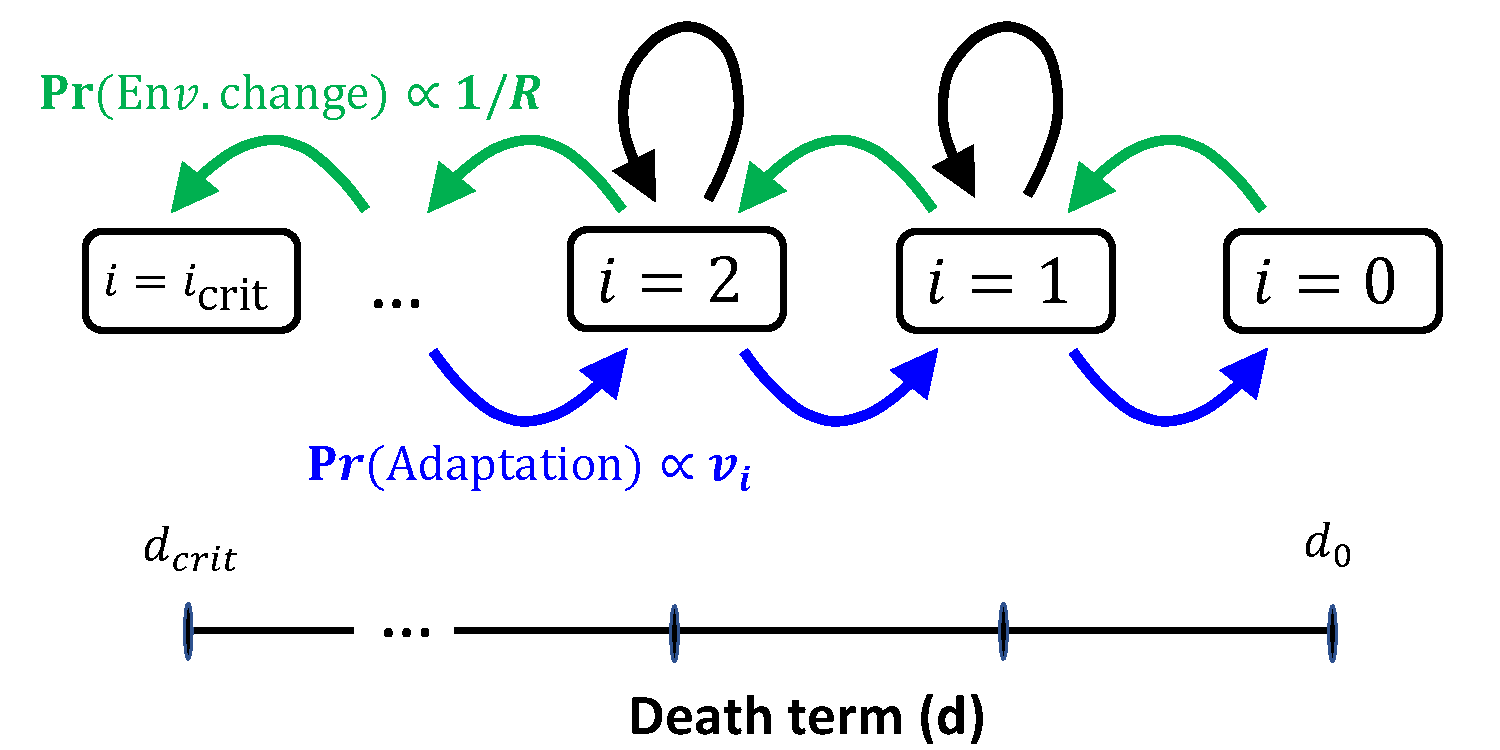
\includegraphics[scale=0.33]{fig_MC_chain_diagram.pdf}
    \caption{Caption}
    \label{fig:my_label}
\end{figure}
\begin{figure}[!h]
    \centering
    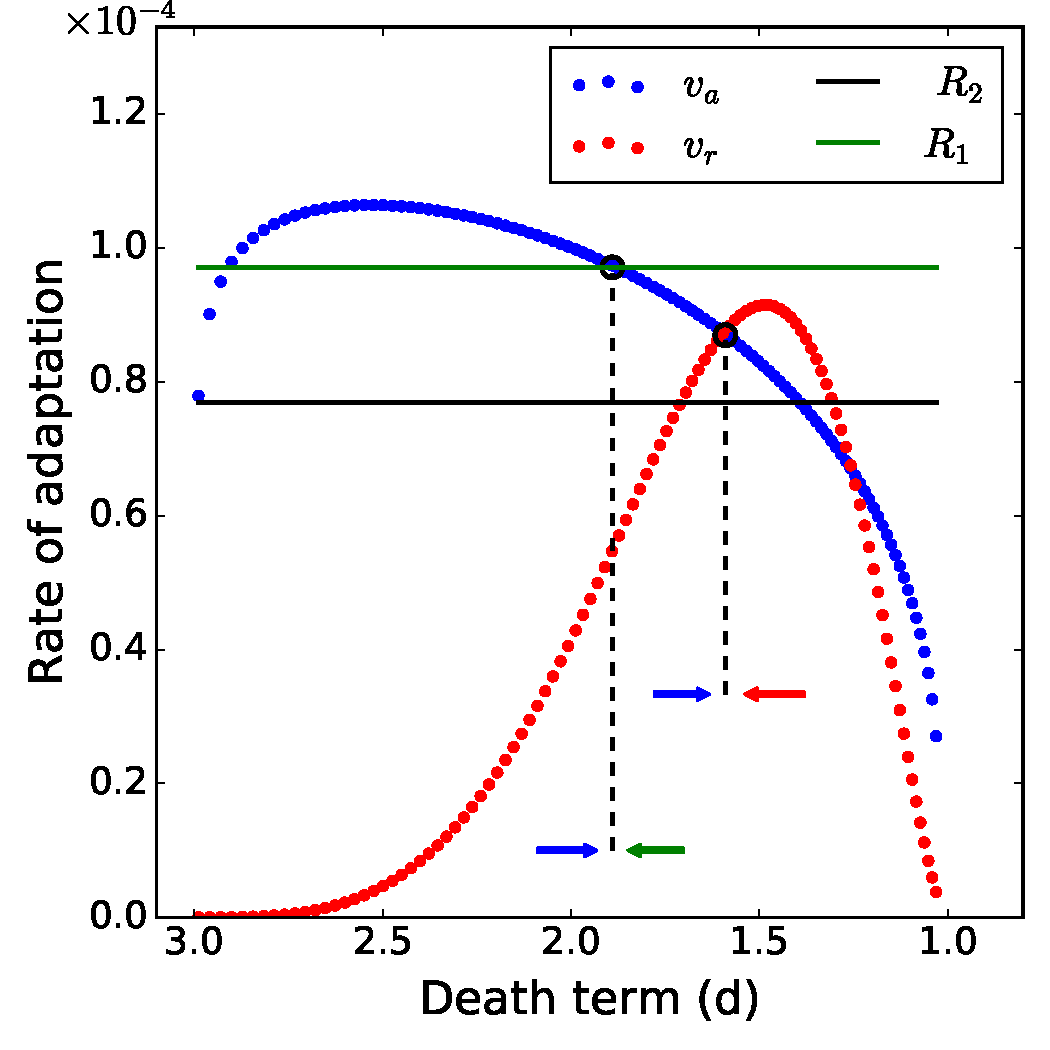
\includegraphics[scale=0.45]{fig_AbsVsRel_MC_chain.pdf}
    \caption{Caption}
    \label{fig:my_label}
\end{figure}
\begin{enumerate}
    \item change in intersection and therefore long-term absolute fitness and possibility of extinction
    
    While these two competing rates of adaptation do not completely control the fate of a given history, they help determine the propensity for extinction under environmental pressures. Therefore it is of great importance to consider what perturbs and might lead to catastrophic deviations in a sample path.
    
    The most obvious consideration, the flexible rather than the regimen, is resource availability or territory size. When can "room to grow" allow for the persistence of a population and, if possible, when call it lead it to perish?
    
    \item intersections are determined by changes in the rates of adaptation; which depend on territory size (among other things)
    
    This can be investigated by considering the intersection of our two adaptation rates, i.e. the adult survival $1/d$, or equivalently the absolute fitness class $i$ that gives $v_a = v_r$. To determine the effect of varying territory size $T$ on the intersection, we need only investigate the respective derivatives of the adaptation rates $\pdv{v_{a}(i)}{T}$ and $\pdv{v_{r}(i)}{T}$ and their respective ordering will determine the movement of the intersection $d^{*},i^{*}$. 
    

    \item dva/dt, dvr/dt
    
    
Here we find that taking the derivative of our rates of adaptation with respect to the territory size, as per our example, that as expected the results are usefully symmetric
\begin{align*}
    \pdv{v_{a}(i)}{T} & \approx \frac{2}{T}  \frac{1}{ \left [ \frac{1}{s_{a}}\ln  \left ( \frac{s_{a}}{U_{a}(i)} \right ) \right ]^2} \\
    \pdv{v_{r}(i)}{T} & \approx \frac{2}{T}  \frac{1}{ \left [ \frac{1}{s_{r}^{*}(i)} \ln \left(\frac{s_{r}^{*}(i)}{U_{r}}\right) \right ]^2}
\end{align*}


    \item ratios, introduce taus and our interpretation of them, and possible inequalities ("possible results" with the intersection because of difference in the derivatives; theoretically we could move in the "wrong" direction)
    
    
This rather clean setup suggests two different approaches, one that explicitly makes use of these derivatives, and required relationships at the intersection of the two curves. Here we find that the movement of the intersection and therefore stationary distribution of absolute fitness is determined by something we will denote as relative “basic mutation timescales” of each trait (as they are referred to in Desai and Fisher, right above eq. 6),

$$\tau_{r}(i) = \left[\frac{1}{s_{r}^{*}(i)}\ln \left(\frac{s_{r}^{*}(i)}{U_{r}}\right)\right]$$ and $$\tau_{a}(i) = \left[\frac{1}{s_{a}}\ln \left(\frac{s_{a}(i)}{U_{a}(i)}\right)\right]$$

Here we find that, theoretically, we may get circumstances such that when $\tau_{r}(i)  < \tau_{a}(i)$ the intersection moves $away$ from the optimum absolute fitness (towards more negative absolute fitness values or greater death-rates), indicating that the competitive trait dominates in such regimes and drives the population towards a worse fitness outcomes. However how often does this occur in practice? 
    
\end{enumerate}

\section{Results}
\begin{itemize}
    \item "Typical" initial parameters related (within the scope of) Desai and Fisher and Jason, Kevin; predicts an un-intuitive result i.e. WRONG DIRECTION.
    
    [Describe the parameters used the papers above].
    
    Introducing these parameters into our Markov-Approximation we find an un-intuitive result. Under the Running out of Mutations assumption ($RM$) and using the "canonical" parameterization, we see that competitive interference is large enough so that increasing available resources actually $decreases$ the absolute fitness of the population population.
    
    \item Why? tau ratio here, show plot.
    
    As seen in the graph above we end up with the theoretically 
    \item So what happens if we drive territory size to infinity to kill off a populations
    \item no, there's an asymptotes (increase risk of extinction, but cannot drive you to extinction)
    \item asymptotes in territory size, biological (buffered by other trait)
    \item balances in the selection and mutation rate, maximal (increase or decrease) in absolute fitness
    \item Analyze some of the results of the ratio; maybe the implicit function of the territory size, prediction of asymptotes
    \item depends on other parameters as well: b, d, etcetera.
    \item heuristics compatible with simulations?
\end{itemize}

The other approach, noticed after finding an apparent asymptotic relationship between the territory size and the intersection of the velocities, creates a function of the inverse with respect to territory size as a function of absolute fitness. The rate of adaptation for both the absolute and relative trait, with respect to log-territory size are linear, that produce a relationship at the intersection of the form
\begin{align*}
    v_{a}(i) & \stackrel{*}{=} v_{r}(i) \\
    2 \tau_{a}(i) \ln (T^*) + \alpha_{a}(i) \tau_{a}(i) & \stackrel{*}{=}
    2 \tau_{r}(i) \ln (T^*) + \alpha_{r}(i) \tau_{r}(i)
\end{align*}
thus inverse with respect to $T$, we generate the required Territory size for a given intersection $T^*(i)$ as
$$ T^{*}(i) =  \exp \left \{-\frac{1}{2} \left[ \frac{\alpha_{a}(i) \tau_{a}(i) - \alpha_{r}(i) \tau_{r}(i)}{ \tau_{a}(i) - \tau_{r}(i)} \right] \right \}$$
    
Here we find that our asymptotes occur where we have equality in time scales, i.e. stagnation in the absolute fitness with respect to the territory size occur at these points (as it freely exists on the full scale for a given absolute fitness value). These points are never achievable unless via initial construction, but come onto play with respect to their generated curvature as bounds for the diminishing returns of territory size.

Fundamentally, however, these were conjectures based on the dynamics of the approximation and nothing else. In order to analyze whether these approximations were valid, we considered the numerical model under restriction of the "timescales" in order to test for confounding factors not included in the current model. This is akin to asking the question of whether we can or cannot completely parameterize the relationship between the changes in the intersection by their difference in fitness and mutation rate or if we are missing something. 

First we will fix the timescales to be initially indistinguishable, and check the change in intersection upon perturbing the mutation rate and selection coefficient. Then, if results here correspond with our conjectures, we would work on completely bounding timescales for the absolute and relative traits, in one direction or the other, for both of the \textit{Running out of Mutations} and \textit{Diminishing Return Epistasis} in order to ascertain resulting variations.

% ----------------------------------------------------------------------------------------
% ----------------------------------------------------------------------------------------
% ----------------------------------------------------------------------------------------

\begin{itemize}
\item From Kevin’s last paper, depends on va vs vr
\item From Jason’s 2017 paper, plots with intersections, now 3 lines: va, vr and environmental change. Walk through all the kinds of intersections that might prevail.
\item vr depends on population density, we solve for local equilibrium density and calculate selection coefficient for that
\item These depend in different ways on T
CAN GET UNINTUITIVE RESULT THAT LARGER T LEADS TO LESS ADAPTED POPULATION
\item Examine using dv/dT, derive taua : taur as critical ratio determining intuitive vs unintuitive direction. In effect this is asking is r<a . We derive these terms from 1/(dv/dT)\^2, but they come out equal to timescales in Desai \& Fisher, i.e. the speed of evolution from mutation.
\item At infinite T, deltaT of course doesn’t matter, curvature toward mattering less for large finite T
For DRE we get the intuitive behavior - need to ask if this is always, or just harder to get unintuitive?
\item Questionable results with RM model, maybe not possible to change the direction for change in intersection as of T. Maybe the curvature/tail of the $v_r$, what are the implications? Possible only in Diminishing returns?
\end{itemize}


Figure 1: plot distribution of states with $v_r$ as attractor, $v_r$ above attractor, $v_r$ below attractor of Markov chain approximation. Use fixed rate of environmental change for persistence.

Figure 2: Distribution of extinction times with different $v_r$ mentioned above, as $T$ varies.

Figure 3: Panel with Figure 1 and 2 with diminishing returns epistasis model, and $v_r$ at attractor.

\begin{figure}[!h]
    \centering
    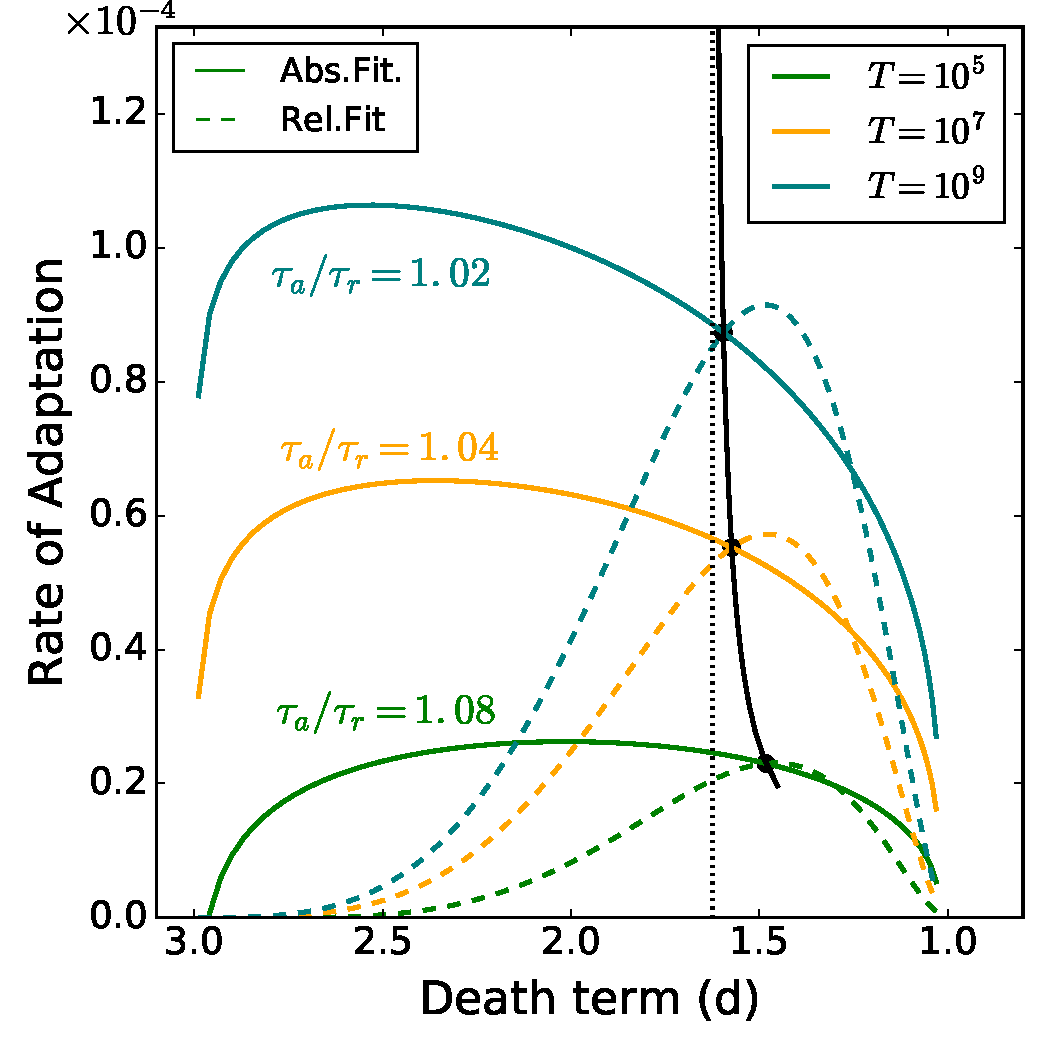
\includegraphics[scale=.45]{fig_decrAbsAdaptTerritorySize.pdf}
    \caption{Absolute and relative rates of adaptation over absolute fitness space and the trace of their intersection points for various values of Territory size $T$.}
    \label{fig:intersectVrVafunctT}
\end{figure}

\section{Discussion}
\textbf{FOURTH PIVOTAL PARAGRAPH}
\\ \\
\begin{itemize}
    \item DR belongs in discussion (we looked at it, see version of graph in supplement), and ultimately, its just harder to get un-intuitive results
\end{itemize}


\textbf{FIFTH PIVOTAL PARAGRAPH}: conclusion goes here
\\ \\
\footnotesize
\bibliographystyle{unsrtnat}
\bibliography{bibliography}

\newpage
\onecolumn
% \appendix \label{sec:appendix}
\begin{appendix}
\section{The quasi-equilibrium population size and density}

In this section, we derive the quasi-equilibrium population size $N^*$ and density $\gamma^*$ for Eq.~\eqref{eq:BMlotNewAd}, in the absence of beneficial mutations with genetic variation only absolute fitness. Thus, we consider Eq.~\eqref{eq:BMlotNewAd} for a set of classes $\{n_{i,j}\}_{i,j}$ with absolute fitnesses $\{d_i\}_i$, competitive ability $c$ and common birth rate $b$; we drop the $j$ index for brevity. 

We first consider the relative change in population size, which is given by
\[
\begin{aligned}
\frac{\Delta N}{N} = \sum_i \frac{n_i}{N} \frac{1}{d_i}\left(1+ \frac{\Delta_s n_i}{n_i}\right)-1 &= \sum_i \frac{p_i}{d_i}\left(1+(e^{-L}+(R_i+A_i)\frac{c}{\bar{c}})\frac{l_{i}}{n_i} U\right)-1\\
&= \sum_i \frac{p_i }{d_i}\left(1+(e^{-L}+(R_i+A_i)) \frac{LU}{N}\right)-1
\end{aligned}
\]
where we use the fact that $c = \bar{c}$ and $l_iU/n_i = LU/N$ to obtain the second line. Furthermore, the terms $R_i$ and $A_i$ of Eq.~\eqref{eq:BMlotCompTerms} are given by 
\[
R_i = \frac{\bar{c}(e^{-l_i} -e^{-L}) }{c+\frac{\bar{c}L-cl_i}{L-l_i}\frac{L-1+e^{-L}}{1-(1+L)e^{-L}}} = (e^{-l_i} -e^{-L} )\frac{1-(1+L)e^{-L}}{L(1-e^{-L})} 
\]
and
\[
A_i = \frac{\bar{c}(1-e^{-l_i})}{\frac{ c l_i (1-e^{-l_i})}{1-(1+l_i)e^{-l_i} }+\frac{\bar{c}L-c l_i}{L-l_i} \left( \frac{L(1-e^{-L})}{1-(1+L)e^{-L}}-\frac{l_i(1-e^{-l_i})}{1-(1+l_i)e^{-l_i}}\right)} = (1-e^{-l_i})\frac{1-(1+L)e^{-L}}{L(1-e^{-L})}
\]
after cancelling out the $c$ terms using $\bar{c}=c$. Thus, 
\[
R_i + A_i = \frac{(1-(1+L)e^{-L})}{L} = \frac{(1-e^{-L})}{L}-e^{-L}.
\]
which allows us to further reduce the right side of $\Delta N/N$,
\[
\begin{aligned}
\frac{\Delta N}{N} &= \sum_i \frac{p_i }{d_i}\left(1+(e^{-L}+\frac{(1-e^{-L})}{L}-e^{-L}) \frac{LU}{N}\right)-1\\
&= \sum_i \frac{p_i }{d_i}\left(1+(1-e^{-L})\frac{U}{N}\right)-1\\
&= \left(1+(1-e^{-L})\frac{U}{N}\right)\frac{1}{d_H}-1\\
&= \left(1+(1-e^{-bN/T})\left(\frac{T}{N}-1\right)\right)\frac{1}{d_H}-1
\end{aligned}
\]
where $d_H$ is the harmonic mean of the $d_i$'s, and $L=bN/T$ has been substituted into the last line. The population size can achieve a quasi-equilibrium state if $d_H$ remains approximately constant over the period require for $\Delta N/N \approx 0$. Then $N^*$ will solve the equation,
\[
0 =\left(1+(1-e^{-bN/T})\left(\frac{T}{N}-1\right)\right)\frac{1}{d_H}-1
\]
Rather than solving for $N^*$, we instead consider $\gamma^* = N^*/T$. Rewriting the above expression with $\gamma = N/T$ and rearranging terms provides
\[
(d_H -1)\gamma = (1-\gamma)(1-e^{-b\gamma}).
\]
The expression has at most two solutions for $0 \leq \gamma \leq 1$; this can be seen from plotting the left and right hand sides. A solution $\gamma^*>0$ will exist if the derivative left-hand side ($d_H-1$) is smaller than the derivative of the right-hand side ($b+1$) at $\gamma =0$. If $d_H-1\geq b+1$, then changes in population size will eventually drive the population extinct. We solve for $\gamma^*$ numerically.
\begin{figure}[h!]
    \centering
    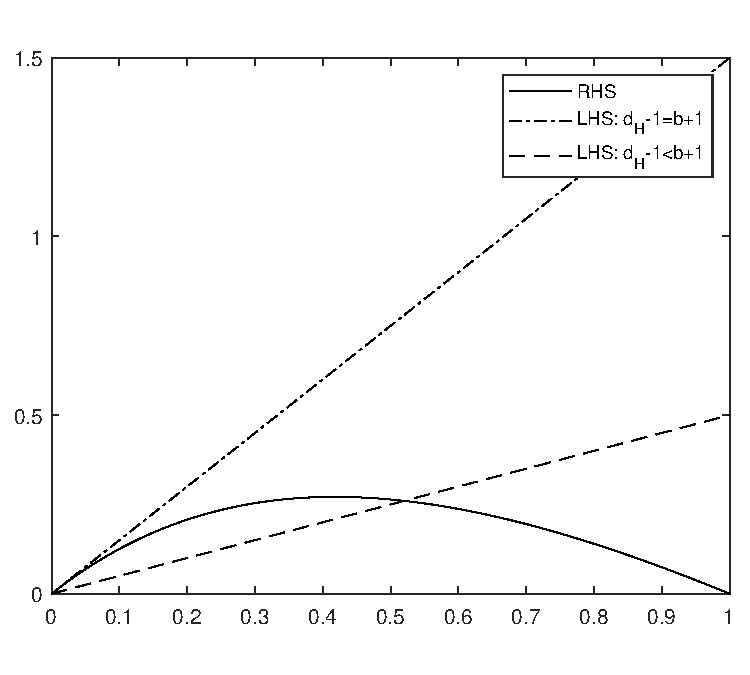
\includegraphics[scale=.6]{densitySoltn.pdf}
    \caption{Possible solutions for quasi-equilibrium's densities.}
    \label{fig:qEdensity}
\end{figure}

\section{Selection coefficients of beneficial mutations in absolute and relative fitness relative traits}

Here we derive the selection coefficient of beneficial mutations in the relative fitness trait. As discussed in \citet[][section 3.2]{bertram2019density}, $c$-selection exhibits a density dependence, and consequently, selection coefficients for beneficial mutations in the $c$ trait will depend on $\gamma$, given in Appendix A. We can determine this relationship by calculating the expected relative change in frequency of a new mutant class arising in a homogeneous population. 

We begin by applying Equation \eqref{eq:SelAdvntg}, and solve for the selective advantage of a mutant class $(i,j)$ as its arises in a population consisting of members from class $(i,j-1)$. This leads to
\[
s_{i,j} \approx \lim_{p_{i,j}\rightarrow 0} \frac{W_{i,j}-\bar{W}}{\bar{W}} = \frac{W_{i,j}-W_{i,j-1}}{W_{i,j-1}}\eval_{p_j=0},
\]
which can be expanded using \eqref{eq:ExpctChngeAbund}. We will drop the $i$ index to simplify the calculations that follow. We also use the fact that $l_j = bn_j/T = b(N/T)(n_j/N) = b\gamma p_j$ and $L=b\gamma$. Given 
\[
\begin{aligned}
W_j = \frac{1}{d}\left[1+\left(e^{-L} +(R_j+A_j)\frac{c_j}{\bar{c}}\right)\frac{l_j}{n_j}U\right] = \frac{1}{d}\left[1+\left(e^{-L} +\frac{c_j}{\bar{c}}R_j+ \frac{c_j}{\bar{c}}A_j)\right)\frac{bU}{T}\right],
\end{aligned}
\]
we substitute for the individual competitive terms that depend on $p_j$ and evaluate at the given value. The first of these terms, $R_j c_j/\bar{c}$, evaluates to
\[
\begin{aligned}
\frac{c_j}{\bar{c}} R_j\eval_{p_j=0} &= \frac{c_j}{\bar{c}} \cdot \frac{\bar{c}e^{-l_{j}}(1-e^{-(L-l_{j})})}{c_j +\frac{\bar{c}L-c_jl_{j}}{L-l_{j}}\frac{L-1+e^{-L}}{1-(1+L)e^{-L}}}\eval_{p_j=0} \\[4pt]
&= 
\frac{c_j(e^{-b\gamma p_j}-e^{-b\gamma})}{c_j +\frac{b\gamma (\bar{c}-c_jp_j)}{b\gamma (1-p_j)}\frac{b\gamma-1+e^{-b\gamma}}{1-(1+b\gamma)e^{-b\gamma}}}\eval_{p_j=0} \\[4pt]
&= \frac{c_j(1-e^{-b\gamma})}{c_j +c_{j-1}\frac{b\gamma-1+e^{-b\gamma}}{1-(1+b\gamma)e^{-b\gamma}}} 
\end{aligned}
\]
We now used the fact that $c_j = (1+s_r)c_{j-1}$ and substitute
\[
\begin{aligned}
\frac{c_j}{\bar{c}}R_j\eval_{p_j=0}&= \frac{(1+s_r)(1-e^{-b\gamma})}{(1+s_r) +\frac{b\gamma-1+e^{-b\gamma}}{1-(1+b\gamma)e^{-b\gamma}}} \\[4pt]
&= \frac{(1+s_r)(1-e^{-b\gamma})}{s_r + \frac{b\gamma(1-e^{-b\gamma})}{1-(1+b\gamma)e^{-b\gamma}}}.\hspace{.8in}
\end{aligned}
\]
For the second competitive term $A_j c_j/\bar{c}$ we have
\[
\begin{aligned}
\frac{c_j}{\bar{c}}A_{j}\eval_{p_j=0} &=  \frac{c_j}{\bar{c}} \cdot \frac{\bar{c}(1-e^{-l_{j}})}{ \frac{c_j l_j(1-e^{-l_{j}})}{1-(1+l_{j})e^{-l_{j}}}+\frac{\bar{c}L-c_jl_{j}}{L-l_{j}}\left(\frac{L(1-e^{-L})}{1-(1+L)e^{-L}}-\frac{l_{j}(1-e^{-l_{j}})}{1-(1+l_{j})e^{-l_{j}}}\right)} \eval_{p_j=0}\\[4pt]
&=  \frac{c_j(1-e^{-b\gamma p_j})}{ \frac{c_jb\gamma p_j(1-e^{-b\gamma p_j})}{1-(1+b\gamma p_j)e^{-b\gamma p_j}}+\frac{b\gamma(\bar{c}-c_jp_j)}{b\gamma(1-p_{j})}\left(\frac{b\gamma(1-e^{-b\gamma})}{1-(1+b\gamma)e^{-b\gamma}}-\frac{b\gamma p_{j}(1-e^{-b\gamma p_{j}})}{1-(1+b\gamma p_{j})e^{-b\gamma p_{j}}}\right)}\eval_{p_j=0}\\[4pt]
&=  0
\end{aligned}
\]
since the numerator of the second line on the right evaluates to zero. This leads to the expression
\begin{equation}
\begin{aligned}
W_j  = \frac{1}{d}\left[1+\left(e^{-L} + \frac{(1+s_r)(1-e^{-b\gamma})}{s_r + \frac{b\gamma(1-e^{-b\gamma})}{1-(1+b\gamma)e^{-b\gamma}}}\right)b(1-\gamma)\right]
\end{aligned}
\end{equation}
where we have substituted $bU/T = b(1-\gamma)$. Next, we compute
\[
\begin{aligned}
W_{j-1} = \frac{1}{d}\left[1+\left(e^{-L} +\frac{c_{j-1}}{\bar{c}}R_{j-1}+ \frac{c_{j-1}}{\bar{c}}A_{j-1})\right)b(1-\gamma)\right],
\end{aligned}
\]
by substituting and evaluating the two competitive terms. This will lead to similar expression to those just obtained, but we find that 
\[
\begin{aligned}
\frac{c_{j-1}}{\bar{c}} R_{j-1}\eval_{p_{j-1}=1} &= \frac{c_{j-1}}{\bar{c}} \cdot \frac{\bar{c}e^{-l_{j-1}}(1-e^{-(L-l_{j-1})})}{c_{j-1} +\frac{\bar{c}L-c_{j-1}l_{j-1}}{L-l_{j-1}}\frac{L-1+e^{-L}}{1-(1+L)e^{-L}}}\eval_{p_{j-1}=1} \\[4pt]
&= 
\frac{c_{j-1}(e^{-b\gamma p_{j-1}}-e^{-b\gamma})}{c_{j-1} +\frac{b\gamma (\bar{c}-c_{j-1}p_{j-1})}{b\gamma (1-p_{j-1})}\frac{b\gamma-1+e^{-b\gamma}}{1-(1+b\gamma)e^{-b\gamma}}}\eval_{p_{j-1}=1} \\[4pt]
&= 0
\end{aligned}
\]
since the numerator of the second line evaluates to $0$, and 
\[
\begin{aligned}
\frac{c_{j-1}}{\bar{c}}A_{j-1}\eval_{p_{j-1}=1} &=  \frac{c_{j-1}}{\bar{c}} \cdot \frac{\bar{c}(1-e^{-l_{j-1}})}{ \frac{c_{j-1}l_{j-1}(1-e^{-l_{j-1}})}{1-(1+l_{j-1})e^{-l_{j-1}}}+\frac{\bar{c}L-c_{j-1}l_{j-1}}{L-l_{j-1}}\left(\frac{L(1-e^{-L})}{1-(1+L)e^{-L}}-\frac{l_{j-1}(1-e^{-l_{j-1}})}{1-(1+l_{j-1})e^{-l_{j-1}}}\right)} \eval_{p_{j-1}=1}\\[4pt]
&=  \frac{c_{j-1}(1-e^{-b\gamma p_{j-1}})}{ \frac{c_{j-1}b\gamma p_{j-1}(1-e^{-b\gamma p_{j-1}})}{1-(1+b\gamma p_{j-1})e^{-b\gamma p_{j-1}}}+\frac{b\gamma(\bar{c}-c_{j-1}p_{j-1})}{b\gamma(1-p_{j-1})}\left(\frac{b\gamma(1-e^{-b\gamma})}{1-(1+b\gamma)e^{-b\gamma}}-\frac{b\gamma p_{j-1}(1-e^{-b\gamma p_{j-1}})}{1-(1+b\gamma p_{j-1})e^{-b\gamma p_{j-1}}}\right)}\eval_{p_{j-1}=1}\\[4pt]
&=  \frac{(1-e^{-b\gamma})}{ \frac{b\gamma(1-e^{-b\gamma })}{1-(1+b\gamma )e^{-b\gamma }})}.
\end{aligned}
\]
Note that the second expression on the right must involves a $0/0$ expression when evaluated. The limit as $p_{j-1}\rightarrow 1$ is meant when going from the second line to the third. Having solved for $(c_{j-1}/\bar{c})R_{j-1}+(c_{j-1}/\bar{c})A_{j-1}$, we arrive to the expression 
\begin{equation}
\begin{aligned}
W_{j-1} =\frac{1}{d}\left[1+\left(e^{-L} + \frac{(1-e^{-b\gamma})}{ \frac{b\gamma(1-e^{-b\gamma })}{1-(1+b\gamma )e^{-b\gamma }}}\right)b(1-\gamma)\right] = \frac{1}{d}\left[1+
(1-e^{-b\gamma })
\frac{(1-\gamma)}{\gamma}\right]
\end{aligned}
\end{equation}
Combining our results for $W_j$ and $W_{j-1}$ provides
\[
\begin{aligned}
\frac{W_{i,j}-W_{i,j-1}}{W_{i,j-1}}\eval_{p_j=0} &= \left( \frac{(1+s_r)(1-e^{-b\gamma})}{s_r + \frac{b\gamma(1-e^{-b\gamma})}{1-(1+b\gamma)e^{-b\gamma}}}- \frac{(1-e^{-b\gamma})}{ \frac{b\gamma(1-e^{-b\gamma })}{1-(1+b\gamma)e^{-b\gamma }}}\right) b(1-\gamma) \left[1+
(1-e^{-b\gamma })
\frac{(1-\gamma)}{\gamma}\right]^{-1}\\[4pt]
&= \left( \frac{(1+s_r)}{1 + \frac{s_r(1-(1+b\gamma)e^{-b\gamma})}{b\gamma(1-e^{-b\gamma})}}- 1\right) (1-(1+b\gamma)e^{-b\gamma })\frac{(1-\gamma)}{\gamma} \left[1+(1-e^{-b\gamma })\frac{(1-\gamma)}{\gamma}\right]^{-1}\\[4pt]
&= \left( \frac{(1+s_r)}{1 + \frac{s_r(1-(1+b\gamma)e^{-b\gamma})}{b\gamma(1-e^{-b\gamma})}}- 1\right)\frac{1-(1+b\gamma)e^{-b\gamma }}{\frac{\gamma}{1-\gamma}+(1-e^{-b\gamma })}\\[4pt]
&= \left( \frac{(1+s_r)-\left(1+ \frac{s_r(1-(1+b\gamma)e^{-b\gamma})}{b\gamma(1-e^{-b\gamma})}\right)}{1+ \frac{s_r(1-(1+b\gamma)e^{-b\gamma})}{b\gamma(1-e^{-b\gamma}}}\right)\frac{1-(1+b\gamma)e^{-b\gamma }}{\frac{\gamma}{1-\gamma}+(1-e^{-b\gamma })}\\[4pt]
&= \left( s_r\cdot\frac{1- \frac{(1-(1+b\gamma)e^{-b\gamma})}{b\gamma(1-e^{-b\gamma})}}{1+ \frac{s_r(1-(1+b\gamma)e^{-b\gamma})}{b\gamma(1-e^{-b\gamma}}}\right)\frac{1-(1+b\gamma)e^{-b\gamma }}{\frac{\gamma}{1-\gamma}+(1-e^{-b\gamma })}\\[4pt]
&= \left( \frac{s_r}{b\gamma(1-e^{-b\gamma})}\cdot\frac{b\gamma-b\gamma e^{-b\gamma}- 1+e^{-b\gamma}+b\gamma e^{-b\gamma}}{1+ \frac{s_r(1-(1+b\gamma)e^{-b\gamma})}{b\gamma(1-e^{-b\gamma})}}\right)\frac{1-(1+b\gamma)e^{-b\gamma }}{\frac{\gamma}{1-\gamma}+(1-e^{-b\gamma })}\\[4pt]
&= s_r \left( \frac{1}{b\gamma(1-e^{-b\gamma})}\cdot\frac{b\gamma -1 +e^{-b\gamma}}{1+ \frac{s_r(1-(1+b\gamma)e^{-b\gamma})}{b\gamma(1-e^{-b\gamma})}}\right)\frac{1-(1+b\gamma)e^{-b\gamma }}{\frac{\gamma}{1-\gamma}+(1-e^{-b\gamma })}\\[4pt]
&= s_r \left( \frac{b\gamma -1 +e^{-b\gamma}}{{s_r(1-(1+b\gamma)e^{-b\gamma})}+{b\gamma(1-e^{-b\gamma})}}\right)\frac{1-(1+b\gamma)e^{-b\gamma }}{\frac{\gamma}{1-\gamma}+(1-e^{-b\gamma })}\\[4pt]
&= s_r \left(\frac{1-\gamma}{\gamma}\right)\left(\frac{1-(1+b\gamma)e^{-b\gamma }}{1+\frac{1-\gamma}{\gamma}(1-e^{-b\gamma })}\right)\left( \frac{b\gamma-1+e^{-b\gamma}}{{s_r(1-(1+b\gamma)e^{-b\gamma})}+{b\gamma(1-e^{-b\gamma})}}\right)\\[4pt]
\end{aligned}
\]
and thus, 
\begin{equation} \label{eq:compSelCoeff}
S_{r}(s_{r};\gamma_{i},b)=\frac{W_{i,j}-W_{i,j-1}}{W_{i,j-1}}\eval_{p_j=0}= s_r \left(\frac{1-\gamma}{\gamma}\right)\left(\frac{1-(1+b\gamma)e^{-b\gamma }}{1+\frac{1-\gamma}{\gamma}(1-e^{-b\gamma })}\right)\left( \frac{b\gamma-1+e^{-b\gamma}}{{s_r(1-(1+b\gamma)e^{-b\gamma})}+{b\gamma(1-e^{-b\gamma})}}\right).
\end{equation}
The first two factors on the right-handside of Eq.~\eqref{eq:compSelCoeff}, have limits
\[
\lim_{\gamma\rightarrow 0} \left(\frac{1-\gamma}{\gamma}\right)\left(\frac{1-(1+b\gamma)e^{-b\gamma }}{1+\frac{1-\gamma}{\gamma}(1-e^{-b\gamma })}\right) = \lim_{\gamma\rightarrow 0} \left(\frac{1-\gamma}{\gamma}\right)\left(\frac{b^2\gamma^2}{1+(1-\gamma)b}\right) = 0
\]
and
\[
\lim_{\gamma\rightarrow 1} \left(\frac{1-\gamma}{\gamma}\right)\left(\frac{1-(1+b\gamma)e^{-b\gamma }}{1+\frac{1-\gamma}{\gamma}(1-e^{-b\gamma })}\right) =  \left(\frac{1-\gamma}{\gamma}\right)\left(\frac{1-(1+b\gamma)e^{-b\gamma }}{1+\frac{1-\gamma}{\gamma}(1-e^{-b\gamma })}\right)\eval_{\gamma=1}=0
\]
indicating that the selection coefficient for beneficial mutations in the $c$-trait are largest for intermediate population densities $\gamma$, but approach zero at low and high population densities, as discussed in \cite{bertram2019density}.

\section{Effect of Territory size $T$ on stalling}
\begin{align*}
    v_{a}(i) & \approx s_{a}^2  \frac{ \ln (T^2  \gamma_{i}^2(b,d,s_{a}) s_{a} U_{a}(i)) }{ \ln^2 \left ( \frac{s_{a}}{U_{a}(i)} \right )} \\ & =
    \left[\frac{1}{s_{a}}\ln \left(\frac{s_{a}}{U_{a}(i)}\right)\right]^{-2} [2\ln (T) +  \ln(\gamma_{i}^2(b,d,s_{a}) s_{a} U_{a}(i))] \\ \\
    v_{r}(i) & \approx s_{r}^{*}(i)^2  \frac{ \ln (T^2) +\ln(  \gamma_{i}^2(b,d,s_{a}) s_{r}^{*}(s_{r};\gamma_{i},b)U_r) }{ \ln^2 \left(\frac{s_{r}^{*}(s_{r};\gamma_{i},b)}{U_{r}}\right)} \\ & = \left[\frac{1}{s_{r}^{*}(i)}\ln \left(\frac{s_{r}^{*}(s_{r};\gamma_{i},b)}{U_{r}}\right)\right]^{-2}  [2\ln (T) +\ln(  \gamma_{i}^2(b,d,s_{a}) s_{r}^{*}(s_{r};\gamma_{i},b)U_r)]
\end{align*}
For simplicity let the linear coefficients with respect to $2\ln(T)$ be $\beta_{a}(i)$ and $\beta_{r}(i)$ respectively, and the additive terms inside the brackets be $\alpha_{a}(i)$ and $\alpha_{r}(i)$. Then with $T = T^*$ at intersection we have with

\begin{align*}
    v_{a}(i) & \stackrel{\Delta}{=} v_{r}(i) \\
    2 \beta_{a}(i) \ln (T^*) + \alpha_{a}(i) \beta_{a}(i) & =
    2 \beta_{r}(i) \ln (T^*) + \alpha_{r}(i) \beta_{r}(i)
\end{align*}
the intersection $T^*$ we have
$$ T^* =  \exp \left \{-\frac{1}{2} \left[ \frac{\alpha_{a}(i) \beta_{a}(i) - \alpha_{r}(i) \beta_{r}(i)}{ \beta_{a}(i) - \beta_{r}(i)} \right] \right \}$$
    
\section{Difference in derivative coefficients at rate intersection}
Let $$\tau_{r}(i) = \left[\frac{1}{s_{r}^{*}(i)}\ln \left(\frac{s_{r}^{*}(s_{r};\gamma_{i},b)}{U_{r}}\right)\right]$$ and $$\tau_{a}(i) = \left[\frac{1}{s_{a}}\ln \left(\frac{s_{a}}{U_{a}(i)}\right)\right]$$

At intersection $v_{a} = v_{r}$ we thus have that $$ \left[\frac{1}{s_{r}^{*}(i)}\ln \left(\frac{s_{r}^{*}(s_{r};\gamma_{i},b)}{U_{r}}\right)\right]^{-2}  \ln (T^2  \gamma_{i}^2(b,d,s_{a}) s_{r}(i) U_{r}) =  \left[\frac{1}{s_{a}}\ln \left(\frac{s_{a}}{U_{a}(i)}\right)\right]^{-2}  \ln (T^2  \gamma_{i}^2(b,d,s_{a}) s_{r}(i) U_{r})$$
and thus


$$ \frac{\ln (T^2  \gamma_{i}^2 s_{a} U_{a}(i))}{\ln (T^2  \gamma_{i}^2 s_{r}(i) U_{r})} \left[ \frac{\ln \left(\frac{s_{r}^{*}(i)}{U_{r}}\right)}{\ln \left(\frac{s_{a}}{U_{a}(i)}\right)} \right]^{2} = \left[\frac{s_{r}^{*}(i)}{s_{a}} \right]^{2}At $$


Now if the derivative with respect to the relative fitness trait is larger than the derivative of the absolute trait, we have 
\begin{align*}
    [\tau_{a}(i)]^{-2} & < [\tau_{r}(i)]^{-2} \\
    \left [ \frac{s_{a}}{\ln \left(\frac{s_{a}}{U_{a}(i)}\right)}\right]^{2} & < \left [ \frac{s_{r}(i)}{\ln \left(\frac{s_{r}(i)}{U_{r}}\right)}\right]^{2} \\
    \left [ \frac{\ln \left(\frac{s_{r}(i)}{U_{r}}\right)}{\ln \left(\frac{s_{a}}{U_{a}(i)}\right)}\right]^{2} & < \left [ \frac{s_{r}(i)}{s_{a}}\right]^{2}
\end{align*}

Stringing these inequalities along at intersection we have
$$ \left [ \frac{\ln \left(\frac{s_{r}(i)}{U_{r}}\right)}{\ln \left(\frac{s_{a}}{U_{a}(i)}\right)}\right]^{2}  < \left [ \frac{s_{r}(i)}{s_{a}}\right]^{2} = \frac{\ln (T^2  \gamma_{i}^2 s_{a} U_{a}(i))}{\ln (T^2  \gamma_{i}^2 s_{r}(i) U_{r})} \left[ \frac{\ln \left(\frac{s_{r}^{*}(i)}{U_{r}}\right)}{\ln \left(\frac{s_{a}}{U_{a}(i)}\right)} \right]^{2}  $$

$$ 1  <  \frac{\tau_{a}}{\tau_{r}} = \frac{\ln (T^2  \gamma_{i}^2 s_{a} U_{a}(i))}{\ln (T^2  \gamma_{i}^2 s_{r}(i) U_{r})} $$

\section{stuff}
solve for 

$$\tau_{r}(i) = \left[\frac{1}{s_{r}^{*}(i)}\ln \left(\frac{s_{r}^{*}(s_{r};\gamma_{i},b)}{U_{r}}\right)\right] < \tau_{a}(i) = \left[\frac{1}{s_{a}}\ln \left(\frac{s_{a}}{U_{a}(i)}\right)\right]$$

$$\frac{1}{s_{r}^{*}(i)}\ln \left(\frac{U_{r}}{s_{r}^{*}(s_{r};\gamma_{i},b)}\right) < \frac{1}{s_{a}}\ln \left(\frac{U_{a}(i)}{s_{a}}\right)$$

$$\log(n) \sim \sum_{k}{1/k}$$

\end{appendix}

\end{document}
